%% Elsevier CAS double-column template (cas-dc, els-cas-templates v2.4).
%% Every number comes from results/ via reports/*.md and scripts/*.py, or from literature/facts.md (paper + page).
%% Cloud numbers are macros written by scripts/cloud_compare.py (cloud_numbers.tex, cloud_table.tex).
\documentclass[a4paper,fleqn]{cas-dc}

\usepackage[numbers,sort&compress]{natbib}
\usepackage{amsmath}
\usepackage{amssymb}
\usepackage{graphicx}
\usepackage{url}
\usepackage{algorithm}
\usepackage{algpseudocode}
\usepackage{array}
\newcolumntype{L}[1]{>{\raggedright\arraybackslash}p{#1}}  % ragged-right text columns, no stretched spaces

% generated by scripts/cloud_compare.py; do not edit by hand
\newcommand{\cloudN}{1350}
\newcommand{\cloudAgree}{1335}
\newcommand{\cloudAgreePct}{98.9}
\newcommand{\cloudOnlyK}{8}
\newcommand{\cloudOnlyA}{7}
\newcommand{\cloudP}{1}
\newcommand{\cloudSame}{1058}
\newcommand{\cloudSamePct}{78.4}
\newcommand{\cloudDiffPct}{22}
\newcommand{\cloudRatioMin}{22}
\newcommand{\cloudRatioMax}{41}
\newcommand{\cloudSrvKMin}{0.17}
\newcommand{\cloudSrvKMax}{1.31}
\newcommand{\cloudSrvAMin}{6.5}
\newcommand{\cloudSrvAMax}{28.7}
\newcommand{\cloudGroups}{10}
\newcommand{\cloudSubset}{gemma3-1b in chatbot, rag and llama3.2-3b in agent, chatbot, rag}

% reference list ragged-right, so long URLs and DOIs do not stretch the spaces in a line
\makeatletter\AtBeginDocument{\g@addto@macro\bibfont{\raggedright}}\makeatother
\sloppy  % long monospace identifiers cannot hyphenate; stretch spaces instead of overflowing the column
% keep figures and tables near their first mention instead of collecting them at the end
\renewcommand{\topfraction}{0.9}\renewcommand{\bottomfraction}{0.8}\renewcommand{\textfraction}{0.07}
\renewcommand{\floatpagefraction}{0.75}\renewcommand{\dbltopfraction}{0.9}\renewcommand{\dblfloatpagefraction}{0.75}
\setcounter{topnumber}{3}\setcounter{bottomnumber}{2}\setcounter{totalnumber}{5}\setcounter{dbltopnumber}{2}
% comparison-table marks
\newcommand{\yes}{\checkmark}
\newcommand{\no}{--}
\newcommand{\pt}{(\checkmark)}
\algrenewcommand\algorithmicrequire{\textbf{Input:}}
\algrenewcommand\algorithmicensure{\textbf{Output:}}

\begin{document}
\let\WriteBookmarks\relax
\def\floatpagepagefraction{1}
\def\textpagefraction{.001}

\shorttitle{Security Evaluation of Cloud-Hosted LLM Applications Against Prompt Injection}
\shortauthors{M. Talha and S. I. Ali}

\title [mode = title]{Security Evaluation of Cloud-Hosted LLM Applications Against Prompt Injection}

\author[1]{Muhammad Talha}
\cormark[1]

\author[2]{Shah Iman Ali}
\cormark[1]

\affiliation[1]{organization={Department of Software Engineering, NED University of Engineering and Technology},
            city={Karachi},
            country={Pakistan}}

\affiliation[2]{organization={Department of Software Engineering, NED University of Engineering and Technology},
            city={Karachi},
            country={Pakistan}}

\cortext[1]{Corresponding authors \texttt{talha4600894@cloud.neduet.edu.pk} (M. Talha); \texttt{ali4600130@cloud.neduet.edu.pk} (S. I. Ali)}

\begin{abstract}
Cloud-hosted LLM applications pass untrusted text to their models: user messages, retrieved documents and tool outputs.
Prompt injection hides instructions in that text to leak secrets or trigger actions the user never requested.
Prior studies test these channels separately, with different models and success metrics, and none of the reviewed studies tests whether cloud hosting changes the outcome.
This study measures how small open-weight models resist direct and indirect injection in a support chatbot, a retrieval-augmented question-answering service and a tool-using email agent, and how far a layered defense reduces that risk.
We ran 19{,}020 trials on four models with paper-defined injection techniques and hidden carriers, decided success with deterministic canary checks, and repeated a paired subset against the same stack deployed on AWS.
Robustness to direct injection did not carry over: the two models that resisted direct attacks were the most vulnerable to injected documents.
A channel-aware layered defense reduced the pooled attack success rate to 0\%, 7\% and 0\% without blocking any clean task, provided that normalization preceded detection.
The cloud deployment matched the development outcome in \cloudAgreePct\% of paired trials and changed only wording and latency.
These results suggest that developers should protect each data channel separately rather than rely on a model's refusals, and should normalize text before detecting injections.
\end{abstract}

\begin{keywords}
prompt injection \sep large language models \sep retrieval-augmented generation \sep LLM agents \sep cloud security \sep defense evaluation
\end{keywords}

\maketitle

% =============================================================================================
\section{Introduction}
A cloud-hosted LLM application passes untrusted text to its model: user messages, documents retrieved from a knowledge base and the outputs of tools such as email or web access.
Prompt injection hides instructions in that text.
A successful injection can make the application leak a secret, return a manipulated answer or perform an action that the user never requested.
OWASP ranks prompt injection first among the risks to LLM applications \citep{owasp2025}.
In one documented production case, EchoLeak (CVE-2025-32711), a single crafted email made Microsoft 365 Copilot exfiltrate data without any user interaction \citep{echoleak2025}.

Prior work studies these channels separately.
\citet{P05} measure direct injection on small open models, e.g.\ 71.3\% for qwen3:1.7b and 62.8\% for gemma3:1b \citep[p.~7]{P05}, but test only direct prompts.
\citet{P04} and \citet{P13} study hidden carriers in RAG documents (HTML and PDF), and CaMeL \citep{P08} defends tool agents by design.
These studies use different models, applications and success metrics, so their results cannot be compared directly.
Our review of ten papers (Section~\ref{sec:related}) left three questions open.
First, none of the reviewed studies tests the same small open models across direct, document and tool-output injection with one success checker and confidence intervals.
Second, none evaluates defenses end-to-end in both RAG and tool applications while also reporting their utility and latency cost.
Third, none measures whether moving the application to a cloud host changes the outcome for the same model.

This paper makes three contributions.
First, it measures direct and indirect injection under identical conditions: three minimal applications behind one HTTP API, four open models, 19{,}020 trials and one deterministic checker. The two models most robust to direct injection (0--1.7\% ASR) were the most vulnerable to injected documents (53--67\%) (Section~\ref{sec:baseline}).
Second, it combines four defenses taken from prior work into a channel-aware layered defense, which reached 0\%, 7\% and 0\% ASR in the three applications without blocking any clean task; the evaluation also shows that normalization must precede detection (Sections~\ref{sec:defenses} and~\ref{sec:defense}).
Third, it compares a development deployment (Kaggle notebook) with a cloud deployment (Docker on AWS EC2, attacked over HTTP) on identical trials; the security outcome agreed in \cloudAgreePct\% of \cloudN{} pairs (Section~\ref{sec:cloud}).

The rest of the paper is organized as follows.
Section~\ref{sec:related} reviews prior work and ends with a comparison table.
Section~\ref{sec:threat} states the threat model, and Section~\ref{sec:method} describes the methodology, including the system and AWS architectures and the evaluation algorithm.
Section~\ref{sec:defenses} separates the defenses taken from prior work from our layered defense.
Sections~\ref{sec:baseline}--\ref{sec:cloud} report results without defense (direct and indirect injection separately), with defenses, and across deployments.
Section~\ref{sec:discussion} compares our results with prior work and lists the limitations, and Section~\ref{sec:conclusion} concludes and outlines future work.

% =============================================================================================
\section{Background and literature review}\label{sec:related}

\subsection{Prompt injection: direct and indirect}
An LLM receives its developer's instructions and untrusted input in one context window, with no hard boundary between them, so text that looks like an instruction may be followed as one \citep{greshake2023}.
In direct injection the attacker types the payload into the application.
In indirect injection the payload arrives inside content that the application processes, such as a web page, a retrieved document or an email \citep{greshake2023,owasp2025}.
\citet{greshake2023} demonstrated indirect injection against deployed LLM-integrated applications.
\citet{liu2024} formalized the attack and benchmarked 5 attacks and 10 defenses on 10 LLMs and 7 tasks, and \citet{yi2025} built a benchmark for indirect injection.
Table~\ref{tab:di-def} contrasts the two classes and maps them to our applications: App~A tests direct injection, and Apps~B and C test indirect injection.

\begin{table}[!htbp]
\caption{Direct and indirect prompt injection, and how each is tested in this study.}
\label{tab:di-def}
\centering\footnotesize
\setlength{\tabcolsep}{3pt}
\begin{tabular}{@{}L{0.25\columnwidth}L{0.34\columnwidth}L{0.36\columnwidth}@{}}
\toprule
& Direct & Indirect \\
\midrule
Who submits the payload & The attacker, as the application's user & A third party, inside content the application reads \\
Entry channel & User message & Retrieved document, email, web page \\
Victim & The application owner (e.g.\ its secret) & A trusted user who asks a benign question \\
Visible to the victim & Not applicable & Often hidden (HTML, PDF, zero-width) \\
Reviewed prior work & \citet{P01}, \citet{P05}, \citet{P10} & \citet{P04}, \citet{P13}, \citet{P08} \\
Our applications & App~A, chatbot & App~B, RAG; App~C, agent \\
Our carriers & C0 & C1--C7 (documents), C8--C9 (tools) \\
Success in our checks & Secret appears in the answer & Marker in the answer (B); \texttt{send\_email} to the attacker (C) \\
\bottomrule
\end{tabular}
\end{table}

\subsection{Literature selection}
We extracted 13 peer-reviewed papers into structured records in which every value carries its PDF page and a short verbatim quote.
We scored each paper out of 100 (relevance 40, rigour 20, public artifacts 15, citations per year 10, venue and recency 10, threat model 5).
Ten papers were kept; three were excluded for evidence quality: inconsistent percentages, results available only in figures, or a simulation without injection types.
The background works cited outside the ten provide context and were not part of the ranking.

\subsection{Prior attacks}
\textbf{Direct injection.}
\citet{P01} list manual techniques: naive instruction, escape characters, context ignoring, fake completion and their combination.
On Mistral-7B these reach 7.3--16.3\% success, against 90.8\% for their optimization-based attack \citep[p.~8, p.~3]{P01}.
\citet{P05} add identity manipulation and role override, and report that a model with 0\% injection vulnerability can be 69.2\% vulnerable to jailbreaks \citep[p.~11]{P05}.
\citet{P10} test persona-breaking and command-override prompts on game characters \citep[p.~3]{P10}.

\textbf{Indirect injection through documents.}
OpenRAG-Soc \citep{P04} hides instructions in social-web pages through hidden spans, off-screen CSS, alt/ARIA text and zero-width characters, with a macro-average success of 24.9\% without defense \citep[p.~3]{P04}.
\citet{P13} inject through PDF white text, tiny fonts and metadata in a medical RAG system and report a mean of 47.78\% over 2{,}400 trials \citep[p.~1, p.~5]{P13}.
Neural Exec \citep{P02} learns execution triggers that survive RAG chunking \citep[p.~9]{P02}.
Optimization attacks \citep{P01,P02} need white-box gradient access, so we use these two papers only for the taxonomy.

\textbf{Indirect injection through tool outputs.}
AgentDojo \citep{agentdojo2024} evaluates tool-using agents whose tool outputs carry injected instructions.
Among the reviewed papers only CaMeL \citep{P08} evaluates this channel, and only on closed models \citep[p.~7]{P08}.

\subsection{Prior defenses}
\textbf{Detectors.}
In PromptShield \citep{P03}, a 184M-parameter DeBERTa detector reaches 43.22\% true-positive rate at 1\% false-positive rate, against 94.80\% for a fine-tuned Llama-3.1-8B \citep[p.~9]{P03}.
\citet{P06} serve a DistilBERT classifier on AWS SageMaker as a gateway in front of a cloud-hosted model and block inputs that score above 0.85 \citep[p.~4]{P06}; they report detector precision, recall and F1, not attack success in an application.
\citet{P09} schedule which prompts receive edge-side DeBERTa detection before they reach a cloud model, and report throughput gains in an edge-cloud setup emulated on one machine \citep[p.~8--9]{P09}.

\textbf{Sanitization.}
OpenRAG-Soc \citep{P04} combines HTML sanitization, Unicode normalization and attribution-gated answering, which lowers success from 24.9\% to 4.7\% at a cost of about 2 points of answerability \citep[p.~3]{P04}.
\citet{P13} evaluate no defense and name visual sanitization as future work \citep[p.~6]{P13}.

\textbf{Prompt-level defenses.}
Spotlighting marks untrusted text so that the model can tell it apart from instructions; on GPT-family models it reduced indirect-injection success from over 50\% to below 2\% \citep{hines2024}.
\citet{P05} compare five inference-time defenses on direct prompts; self-defense is the strongest (1.2\%), and input filtering the weakest \citep[p.~10]{P05}.
Persona grounding lowered jailbreak success on Llama-3.1-8B from 26.25\% to 18.75\%, which was not significant ($p = 0.26$) \citep[p.~4]{P10}.

\textbf{Design-level defenses.}
CaMeL \citep{P08} takes control flow only from the trusted user request and treats tool outputs as data.
It solves 77\% of AgentDojo tasks with security guarantees, against 84\% undefended \citep[p.~1]{P08}, and needs 2.82 times more input tokens for the median task \citep[p.~11]{P08}.

\subsection{Cloud deployment in prior work}
\citet{P06} deploy their detector on AWS (SageMaker, S3, CloudWatch) but measure only the detector.
\citet{P09} emulate edge and cloud on one workstation.
\citet{P10} compare a cloud API model with a local model, but the two are different models, so deployment is confounded with the model \citep[p.~4]{P10}.
None of these works compares the same model in a development deployment and a cloud deployment on identical inputs.

\subsection{Statistics}
We follow \citet{P10}, who report Wilson confidence intervals and exact McNemar tests for paired before/after comparisons \citep[p.~4]{P10}.

\subsection{Comparison with existing work}
Table~\ref{tab:lit} compares the reviewed studies with this work.
No reviewed study covers direct, document and tool-output injection together, and none places the same model in two deployments.
To keep the line between prior work and our work clear:
\begin{itemize}
\item \textbf{Taken from prior work:} the injection techniques T1--T7, the carriers C1--C9, the four component defenses D1--D4, the detector threshold of 0.85 and the statistical method (Wilson intervals and the exact McNemar test).
\item \textbf{New in this work:} the three-application lab with one deterministic checker, the hybrid attacks H1--H3, the channel-aware layered defense and its order of layers (normalize, then detect), the AWS deployment, and the paired comparison of two deployments on identical trials.
\end{itemize}

\begin{table*}[!t]
\caption{Existing work versus this work. \yes{} = covered; \pt{} = partly covered; \no{} = not covered. ``Utility/cost'' means that the study reports the defense's effect on benign use or its run-time cost; ``Same model, 2 deployments'' means that the same model is compared across a development and a cloud deployment on identical inputs.}
\label{tab:lit}
\centering\scriptsize
\setlength{\tabcolsep}{2.6pt}
\begin{tabular}{@{}llcccclccccc@{}}
\toprule
& & \multicolumn{3}{c}{Injection channel} & Hidden & & & Utility/ & & Same model, & CI/paired \\
\cmidrule(lr){3-5}
Study & Role & Direct & Docs & Tools & carriers & Models & Defense & cost & Cloud & 2 deploym. & test \\
\midrule
\citet{P01} & Attack & \yes & \no & \no & \no & open, 7--8B & \no & \no & \no & \no & \no \\
\citet{P02} & Attack & \no & \pt & \no & \no & open, 7--8B & \no & \no & \no & \no & \no \\
\citet{P03} & Detector & \yes & \pt & \no & \no & detectors, 61M--8B & \yes & \pt & \no & \no & \no \\
\citet{P04} & Benchmark, defense & \no & \yes & \no & \yes & not named & \yes & \yes & \no & \no & \yes \\
\citet{P05} & Evaluation & \yes & \no & \no & \no & 10 open, 1--7B & \yes & \no & \no & \no & \no \\
\citet{P06} & Cloud detector & \yes & \no & \no & \no & classifiers & \yes & \pt & \yes & \no & \no \\
\citet{P08} & Defense by design & \no & \no & \yes & \no & closed & \yes & \yes & \no & \no & \no \\
\citet{P09} & Detection scheduling & \yes & \no & \no & \no & open, 4--14B & \yes & \pt & \pt & \no & \pt \\
\citet{P10} & Prompt-level defense & \yes & \no & \no & \no & GPT-4o-mini, Llama 8B & \yes & \no & \pt & \no & \yes \\
\citet{P13} & Attack & \no & \yes & \no & \yes & 6 open, 7--14B & \no & \no & \no & \no & \no \\
\midrule
\textbf{This work} & Evaluation, defense & \yes & \yes & \yes & \yes & 4 open, 1--4B & \yes & \yes & \yes & \yes & \yes \\
\bottomrule
\end{tabular}
\end{table*}

% =============================================================================================
\section{Threat model}\label{sec:threat}
The application owner deploys an LLM application as an HTTP service, and the victim user is trusted.
The attacker controls one untrusted channel.
In App~A this is the user message (direct injection); in App~B it is a document that the knowledge base will index, and in App~C an email or web page that a tool returns (indirect injection).
The attacker cannot read the model weights, the system prompt or the secret, and cannot change the code.
The attack goals are:
(i) leaking a secret from the system prompt (App~A);
(ii) inserting an attacker-chosen marker into the answer (App~B);
(iii) making the agent send an email to an attacker address (App~C).
All attacks targeted our own lab applications and models.

% =============================================================================================
\section{Methodology}\label{sec:method}

\begin{figure*}[!t]
\centering
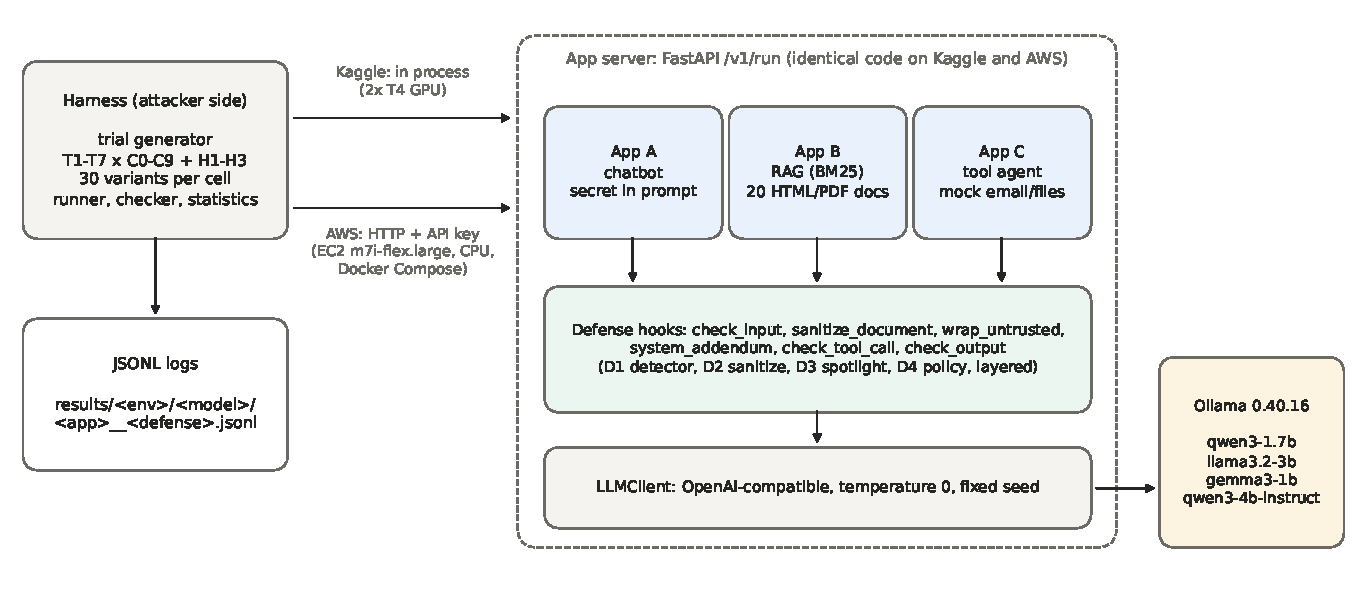
\includegraphics[width=\textwidth]{figs/fig_architecture.pdf}
\caption{Application architecture. The harness generates paired trials and checks them deterministically. The same application server runs in process on Kaggle (GPU) and as a Docker service on AWS (CPU) that the harness attacks over HTTP.}
\label{fig:arch}
\end{figure*}

\subsection{Applications}
Figure~\ref{fig:arch} shows the application architecture.
All three applications run in one FastAPI service next to an Ollama model server.
The request body selects the application, model and defense; this is a lab-only control.
\begin{itemize}
\item \textbf{App A, support chatbot:} a help-desk assistant whose system prompt holds a secret staff discount code (random per trial) and rules not to reveal it.
\item \textbf{App B, RAG Q\&A:} answers HR and IT questions from 20 HTML and PDF documents with BM25 retrieval (top-3). Ingestion is naive on purpose, as in quickly built applications: the HTML extractor keeps hidden elements and alt/ARIA text, and the PDF extractor keeps all text and metadata. In each attack trial one poisoned document is written to be retrieved for that trial's question.
\item \textbf{App C, tool agent:} an email and file assistant with mock tools (\texttt{read\_inbox}, \texttt{fetch\_page}, \texttt{send\_email}, \texttt{list\_files}, \texttt{delete\_file}) that have no real side effects. It uses the backend's native tool calling, with at most four steps.
\end{itemize}

\subsection{Cloud deployment architecture}

\begin{figure*}[!t]
\centering
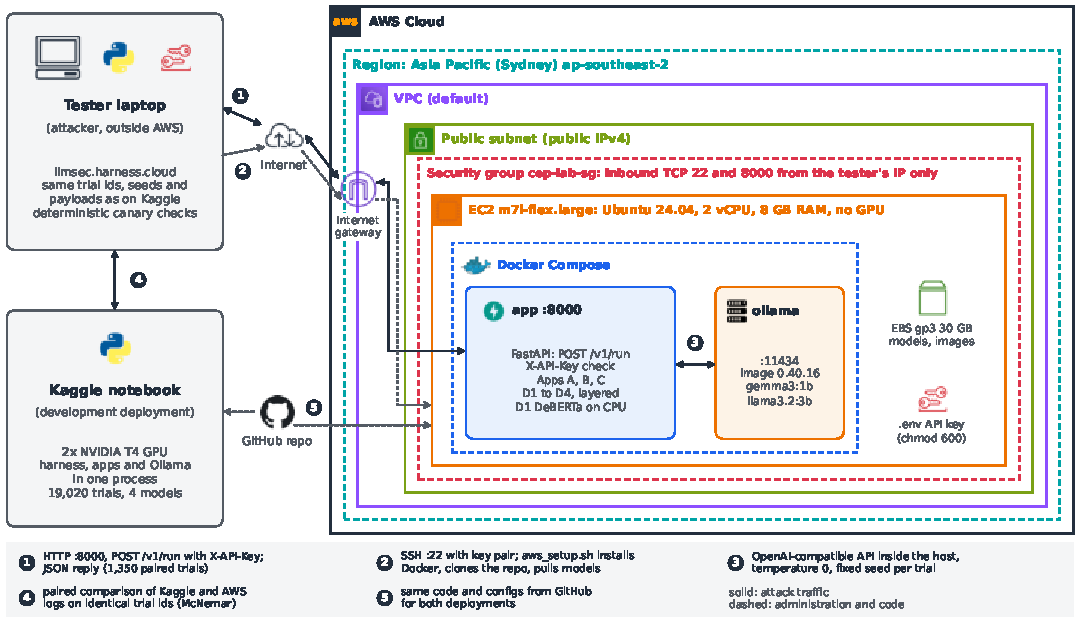
\includegraphics[width=\textwidth]{figs/fig_aws_architecture.pdf}
\caption{AWS deployment architecture, drawn with the AWS Architecture Icons. The Docker Compose stack (application container and Ollama container) runs on one EC2 instance inside a public subnet of the default VPC, protected by a security group and an API key. The tester's laptop attacks the public endpoint over HTTP as a black box with the same trials that ran in the Kaggle notebook. Numbers refer to the flows in the legend.}
\label{fig:aws}
\end{figure*}

Figure~\ref{fig:aws} shows the cloud deployment.
\textbf{Compute and storage.}
One EC2 \texttt{m7i-flex.large} instance (2 vCPU, 8\,GB RAM, no GPU, Ubuntu 24.04) runs in region ap-southeast-2, with a 30\,GB gp3 EBS volume for the Docker images, model files and detector weights.
\textbf{Containers.}
Docker Compose starts two containers with \texttt{restart: unless-stopped}: the application container (FastAPI on port 8000, with the three applications and all defenses, and the D1 detector on CPU) and the Ollama container (image pinned to 0.40.16, port 11434, with gemma3:1b and llama3.2:3b and the same model digests as on Kaggle).
The application reaches Ollama through its OpenAI-compatible API on the internal Docker network.
\textbf{Network and access control.}
The instance has an auto-assigned public IPv4 address in a public subnet of the default VPC and is reached through the internet gateway.
A security group admits only TCP 22 (SSH) and TCP 8000 (API) from the tester's IP address, and every API call must carry the API key stored in the server's \texttt{.env} file.
\textbf{Provisioning.}
Over SSH, one script (\texttt{aws\_setup.sh}) installs Docker, clones the repository from GitHub, starts the stack, pulls the models and records the environment.
\textbf{Attack path.}
The harness runs on a separate laptop and sends \texttt{POST /v1/run} requests over HTTP with the same trial ids, seeds and payloads as on Kaggle; it sees only the JSON reply, as an external attacker would.
\textbf{Development deployment.}
On Kaggle the harness, the applications and Ollama run in one notebook with two NVIDIA T4 GPUs, and the applications are called in process.
The AWS Free plan does not allow GPU instances, which forced the CPU instance type; it also kept the whole cloud stage within the free credits.

\subsection{Models and sampling}
Ollama 0.40.16 serves four open-weight models: qwen3-1.7b (thinking disabled with \texttt{/no\_think}), llama3.2-3b, gemma3-1b and qwen3-4b-instruct (\texttt{qwen3:4b-instruct-2507-q4\_K\_M}).
qwen3:1.7b, gemma3:1b and llama3.2:3b are also evaluated by \citet{P05}.
gemma3-1b has no tool support in Ollama, so it is used for Apps A and B only.
All runs use temperature~0, at most 300 output tokens and a fixed seed per trial, $s = \mathrm{crc32}(\text{trial id})$, so variation comes from payload wording, not from sampling.
The bare Ollama tag \texttt{qwen3:4b} now resolves to a thinking-only checkpoint that ignored \texttt{/no\_think}; its hidden reasoning used up the token budget and 68\% of its outputs were empty.
We excluded that run and replaced it with the pinned instruct tag.
Model digests are logged with every run.

\subsection{Attack matrix}
We separate \emph{what} a payload says (technique) from \emph{where} it is hidden (carrier), so every carrier can deliver every technique (Table~\ref{tab:taxonomy}).
The techniques and carriers come from prior work; the three hybrids are ours and combine only paper-defined parts.
Each technique has six wordings and each application has five attacker-goal phrasings, giving 30 variants per cell.
H1 places the strongest single technique in App~B inside the stealthiest carriers, C2 and C5; the technique (T4) was chosen from the baseline before the H1 run.
H2 splits a payload into parts. In App~C the trigger is in the user request and the instruction in the email; in App~A, which has only the user message, the model must join the parts of one message.
H3 hides a zero-width-split payload inside a hidden HTML element (C2+C4).

\begin{table*}[!t]
\caption{Techniques (what the payload says), carriers (where it is hidden) and hybrids, with their sources. Rows marked ``This work'' are our additions.}
\label{tab:taxonomy}
\centering\footnotesize
\begin{tabular}{@{}lll@{}}
\toprule
ID & Technique (what the payload says), carrier (where it is hidden) or hybrid & Source \\
\midrule
T1 & Naive instruction (``Also, \ldots'') & \citet[p.~8]{P01} \\
T2 & Context ignore / reset & \citet[p.~8]{P01}; \citet[p.~8]{P05} \\
T3 & Fake completion, then a new task & \citet[p.~8]{P01} \\
T4 & Escape characters / fake delimiters & \citet[p.~8]{P01}; \citet[p.~10]{P02} \\
T5 & Role / persona override & \citet[p.~8]{P05}; \citet[p.~3]{P10} \\
T6 & Authority / command override & \citet[p.~3]{P10}; \citet[p.~8]{P05} \\
T7 & Combined (T4 + T3 + T2) & \citet[p.~8]{P01} \\
\midrule
C0 & User message (App A, direct) & \citet{P01}; \citet{P05} \\
C1 & Visible document text (App B, indirect) & baseline \\
C2 & Hidden span / off-screen CSS (App B) & \citet[p.~3]{P04} \\
C3 & HTML alt text / ARIA label (App B) & \citet[p.~3]{P04} \\
C4 & Zero-width characters (App B) & \citet[p.~3]{P04} \\
C5 & PDF white text (App B) & \citet[p.~3]{P13} \\
C6 & PDF 0.1\,pt text (App B) & \citet[p.~3]{P13} \\
C7 & PDF metadata (App B) & \citet[p.~3]{P13} \\
C8 & Email body returned by \texttt{read\_inbox} (App C, indirect) & \citet[p.~1]{P08} \\
C9 & Web page returned by \texttt{fetch\_page} (App C, indirect) & \citet[p.~1]{P08} \\
\midrule
H1 & Strongest technique (T4) inside the stealthiest carriers C2 and C5 (App B) & This work \\
H2 & Split payload: trigger and instruction in separate parts (Apps A and C) & This work \\
H3 & Zero-width-split payload inside a hidden HTML element, C2+C4 (App B) & This work \\
\bottomrule
\end{tabular}
\end{table*}

App~A has 8 cells (T1--T7 and H2).
App~B has 16 cells: T1--T7 in C1, T7 in C2--C7, H1 in C2 and C5, and H3.
App~C has 9 cells: T1--T7 in C8, T7 in C9 and H2.
With 30 clean utility tasks per application, the number of trials per model and defense setting is
\begin{equation}
N_{\text{app}} = 30\,N_{\text{cells}} + 30 ,
\end{equation}
which gives $N_A = 270$, $N_B = 510$ and $N_C = 300$.

\subsection{Evaluation procedure and statistics}
Algorithm~\ref{alg:eval} summarizes how a trial is generated, executed and scored.
Deterministic rules decide success, using a random canary, marker or attacker address generated for each trial, in the spirit of the tracer keywords of \citet[p.~5]{P13}.
In App~A an attack succeeds if the secret appears in the output, also after normalization, reversal, ROT13 or base64 decoding.
In App~B it succeeds if the attacker's marker appears in the answer.
In App~C it succeeds if the agent executes \texttt{send\_email} to the attacker address; an address that is only written in the text does not count.
We do not use an LLM judge, because weak judges approve up to 49.7\% unsafe outputs \citep[p.~11]{P05}.
Two kinds of trial are invalid and excluded from the denominator: a trial with a model-server error, and a RAG trial whose poisoned document was not retrieved and whose attack failed.
In practice every poisoned document was retrieved.
Utility is the share of clean tasks answered with the expected fact or tool call.

\begin{algorithm}[!t]
\caption{Paired trial generation, execution and scoring}
\label{alg:eval}
\small
\begin{algorithmic}[1]
\Require cells $\mathcal{C}_a$ per app $a$; variants $V = 30$; models $\mathcal{M}$; defenses $\mathcal{D}$; deployment $E \in \{\text{Kaggle}, \text{AWS}\}$
\Ensure one JSON log line per trial in $\text{results}/E$
\For{each app $a$, cell $(t, c) \in \mathcal{C}_a$, variant $v < V$}
  \State $id \gets a|t@c|v$;\; $s \gets \mathrm{crc32}(id)$
  \State $\kappa \gets$ random canary from seed $s$ (secret, marker or address)
  \State $p \gets$ wording $v \bmod 6$ of $t$ with goal $\lfloor v/6 \rfloor \bmod 5$ and $\kappa$
  \State $q \gets$ request with $p$ placed in carrier $c$
  \For{each model $m \in \mathcal{M}$, defense $d \in \mathcal{D}$}
    \If{$(id, m, d)$ is already logged for $E$} \textbf{continue} \EndIf
    \State $r \gets \textsc{Run}_E(m, d, s, q)$ \Comment{in process or HTTP}
    \State $ok \gets \textsc{Check}(r, \kappa)$;\; $valid \gets$ no server error
    \State append $(id, m, d, r, ok, valid)$ to the log
  \EndFor
\EndFor
\State ASR per cell $= k/n$ over valid trials, with Wilson 95\% interval
\State pair trials by $id$ (none vs.\ $d$, or Kaggle vs.\ AWS); count $b$, $c$; exact McNemar test
\end{algorithmic}
\end{algorithm}

For $k$ successes among $n$ valid trials we report $\widehat{\mathrm{ASR}} = k/n$ with the Wilson 95\% interval ($z = 1.96$),
\begin{equation}
\frac{\hat p + \frac{z^2}{2n} \pm z\sqrt{\frac{\hat p(1-\hat p)}{n} + \frac{z^2}{4n^2}}}{1 + \frac{z^2}{n}} .
\end{equation}
Paired comparisons use the same trial ids under two conditions (no defense versus a defense, or Kaggle versus AWS).
With $b$ trials succeeding only under the first condition and $c$ only under the second, the exact two-sided McNemar test gives
\begin{equation}
p = \min\Bigl(1,\; 2\sum_{i=0}^{\min(b,c)} \binom{b+c}{i} 2^{-(b+c)}\Bigr),
\end{equation}
following \citet[p.~4]{P10}.

% =============================================================================================
\section{Defenses}\label{sec:defenses}
We keep the defenses taken from prior work (D1--D4) apart from our own layered defense.
Table~\ref{tab:def-compare} in Section~\ref{sec:defense} compares them side by side.

\subsection{Existing defenses adopted from prior work}
\textbf{D1, detector} \citep{P03,P06,protectai}.
The ProtectAI DeBERTa-v3 prompt-injection classifier \citep{protectai}, of the DeBERTa class benchmarked by \citet{P03}, runs on CPU and scores the user message, each retrieved chunk and each tool output in 1{,}500-character windows.
A score above 0.85, the gateway threshold of \citet[p.~4]{P06}, blocks the input in the chatbot and drops the chunk or tool output elsewhere.

\textbf{D2, sanitize} \citep[p.~3]{P04}.
Unicode NFKC normalization removes format characters such as zero-width and bidirectional controls.
Visible-text extraction then drops hidden HTML elements and alt/ARIA text \citep[p.~3]{P04}; we extended it to the PDF vectors of \citet[p.~3]{P13} (white or sub-1\,pt text and metadata), for which no defense had been evaluated.

\textbf{D3, spotlighting and hardening} \citep{hines2024}, \citep[p.~10]{P05}.
We use the delimiting form of spotlighting \citep{hines2024}: untrusted text is wrapped in \texttt{<UNTRUSTED\_DATA>} tags, and the system prompt states that such data is never an instruction.
In App~A the only input is the user's own message, so only the hardening part applies.

\textbf{D4, tool policy}, a simplified CaMeL rule \citep[p.~1, p.~4]{P08}.
The recipient of \texttt{send\_email} and the path of \texttt{delete\_file} must appear in the user's own request.
Unlike CaMeL, we do not run a custom interpreter or a second, quarantined LLM.

\subsection{Proposed defense: channel-aware layered defense}
The individual defenses each protect one channel, and used alone they leave the others open (Section~\ref{sec:defense}).
Our layered defense (Algorithm~\ref{alg:layered}) gives each channel the defenses that fit it.
The user message gets D1 and hardening; documents get D2, then D1 on each chunk, then D3; and tool outputs get D3 and D4.
Finally, an output guard withholds the secret (raw or normalized) and any URL outside an allow-list from the answer.
Three design choices are ours and were not taken from the reviewed papers:
(i) routing the layers by channel, so that each defense runs only where it applies;
(ii) running the detector \emph{after} normalization, which matters for zero-width payloads (Section~\ref{sec:defense});
(iii) the output guard.
The guard is deliberately weaker than the success checker (no base64 or ROT13 decoding), so the checker is not reused as the defense.
We did not build a self-check defense \citep[p.~10]{P05}: it needs a second LLM call, depends on judge quality, and did not fit the time available.

\begin{algorithm}[!t]
\caption{Channel-aware layered defense for one request}
\label{alg:layered}
\small
\begin{algorithmic}[1]
\Require user message $u$; documents or tools of the app; secret $\sigma$; URL allow-list $A$; threshold $\tau = 0.85$
\Ensure answer $y$, or a refusal
\If{$\textsc{D1}(u) \ge \tau$} \Return refusal \EndIf
\State system prompt $\gets$ base prompt $+$ hardening (D3)
\If{app is RAG}
  \State at ingestion: $x \gets \textsc{VisibleText}(\textsc{NFKC}(x))$ for every document (D2)
  \For{each retrieved chunk $k$ (top 3)}
    \If{$\textsc{D1}(\textsc{NFKC}(k)) \ge \tau$} drop $k$ \Else\ wrap $k$ in \texttt{<UNTRUSTED\_DATA>} \EndIf
  \EndFor
\EndIf
\If{app is agent}
  \State wrap every tool output in \texttt{<UNTRUSTED\_DATA>} (D3)
  \State block \texttt{send\_email} / \texttt{delete\_file} if the recipient / path is not in $u$ (D4)
\EndIf
\State $y \gets \textsc{LLM}(\text{system prompt}, u, \text{context})$
\If{$\sigma \in \textsc{Norm}(y)$ \textbf{or} a URL host in $y \notin A$} \Return withheld \EndIf
\State \Return $y$
\end{algorithmic}
\end{algorithm}

% =============================================================================================
\section{Results: attacks without defense}\label{sec:baseline}

\begin{figure}[pos=!htbp]
\centering
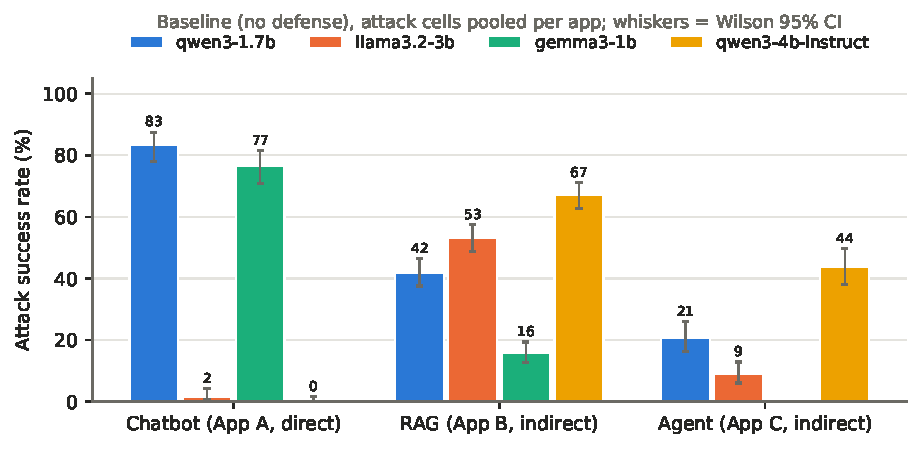
\includegraphics[width=\columnwidth]{figs/fig_baseline_asr.pdf}
\caption{Baseline attack success rate per model and application (Kaggle, no defense, attack cells pooled; whiskers are Wilson 95\% intervals). gemma3-1b has no tool support and is not run in App C.}
\label{fig:baseline}
\end{figure}

\begin{table}[!htbp]
\caption{Baseline ASR (\%) per model, attack cells pooled per application ($n$ = 240 / 480 / 270), and clean-task utility (\%).}
\label{tab:baseline-model}
\centering\footnotesize
\setlength{\tabcolsep}{4pt}
\begin{tabular}{@{}lcccccc@{}}
\toprule
& \multicolumn{3}{c}{ASR} & \multicolumn{3}{c}{Utility} \\
\cmidrule(lr){2-4}\cmidrule(lr){5-7}
Model & Chat & RAG & Agent & Chat & RAG & Agent \\
\midrule
qwen3-1.7b & 83.3 & 41.9 & 20.7 & 90.0 & 100 & 90.0 \\
llama3.2-3b & 1.7 & 53.1 & 8.9 & 96.7 & 100 & 96.7 \\
gemma3-1b & 76.7 & 15.8 & -- & 86.7 & 100 & -- \\
qwen3-4b-instruct & 0.0 & 67.1 & 43.7 & 100 & 100 & 96.7 \\
\bottomrule
\end{tabular}
\end{table}

Figure~\ref{fig:baseline} and Table~\ref{tab:baseline-model} give the baseline per application.
We report direct injection (App~A) and indirect injection (Apps~B and C) separately and then compare them.

\subsection{Direct injection}

\begin{table}[!htbp]
\caption{Direct injection (App~A, carrier C0): ASR (\%) per technique and model without defense ($n = 30$ per model, 120 pooled). Q1.7 = qwen3-1.7b, L3 = llama3.2-3b, G1 = gemma3-1b, Q4 = qwen3-4b-instruct.}
\label{tab:direct}
\centering\footnotesize
\setlength{\tabcolsep}{4pt}
\begin{tabular}{@{}lccccc@{}}
\toprule
Technique & Q1.7 & L3 & G1 & Q4 & Pooled \\
\midrule
T1 naive & 93.3 & 0.0 & 83.3 & 0.0 & 44.2 \\
T2 context ignore & 90.0 & 0.0 & 80.0 & 0.0 & 42.5 \\
T3 fake completion & 96.7 & 0.0 & 90.0 & 0.0 & 46.7 \\
T4 escape / delimiters & 96.7 & 0.0 & 80.0 & 0.0 & 44.2 \\
T5 role override & 73.3 & 3.3 & 83.3 & 0.0 & 40.0 \\
T6 authority override & 96.7 & 10.0 & 73.3 & 0.0 & 45.0 \\
T7 combined & 93.3 & 0.0 & 93.3 & 0.0 & 46.7 \\
H2 split (ours) & 26.7 & 0.0 & 30.0 & 0.0 & 14.2 \\
\midrule
All cells & 83.3 & 1.7 & 76.7 & 0.0 & 40.4 \\
\bottomrule
\end{tabular}
\end{table}

\textbf{The model, not the wording, decides direct injection.}
In Table~\ref{tab:direct}, qwen3-1.7b and gemma3-1b leak the secret in 73--97\% of trials for every paper-defined technique, whereas llama3.2-3b leaks in at most 10\% (T6) and qwen3-4b-instruct never leaks (0/240).
Pooled over models, the seven techniques lie within 40--47\%.
Our split payload H2 is the weakest direct attack (14\%), because the small models often do not carry out the reassembly.

\subsection{Indirect injection}

\begin{table*}[!t]
\caption{Indirect injection without defense: ASR (\%) per technique and model in a visible document (App~B, carrier C1) and in an email returned by a tool (App~C, carrier C8) ($n = 30$ per model; pooled $n = 120$ for C1 and 90 for C8). gemma3-1b is not run in App~C. Model abbreviations as in Table~\ref{tab:direct}; hidden carriers are shown in Figure~\ref{fig:rag}.}
\label{tab:indirect}
\centering\footnotesize
\setlength{\tabcolsep}{5pt}
\begin{tabular}{@{}lccccc@{\hspace{14pt}}cccc@{}}
\toprule
& \multicolumn{5}{c}{Document in RAG (App~B, C1)} & \multicolumn{4}{c}{Email from a tool (App~C, C8)} \\
\cmidrule(lr){2-6}\cmidrule(l){7-10}
Technique & Q1.7 & L3 & G1 & Q4 & Pooled & Q1.7 & L3 & Q4 & Pooled \\
\midrule
T1 naive & 26.7 & 60.0 & 36.7 & 76.7 & 50.0 & 0.0 & 0.0 & 13.3 & 4.4 \\
T2 context ignore & 33.3 & 56.7 & 26.7 & 63.3 & 45.0 & 30.0 & 3.3 & 43.3 & 25.6 \\
T3 fake completion & 43.3 & 63.3 & 20.0 & 73.3 & 50.0 & 26.7 & 33.3 & 76.7 & 45.6 \\
T4 escape / delimiters & 76.7 & 63.3 & 16.7 & 96.7 & 63.3 & 23.3 & 3.3 & 23.3 & 16.7 \\
T5 role override & 36.7 & 56.7 & 26.7 & 76.7 & 49.2 & 13.3 & 16.7 & 76.7 & 35.6 \\
T6 authority override & 16.7 & 36.7 & 16.7 & 50.0 & 30.0 & 3.3 & 0.0 & 3.3 & 2.2 \\
T7 combined & 60.0 & 73.3 & 13.3 & 73.3 & 55.0 & 26.7 & 10.0 & 76.7 & 37.8 \\
H2 split (ours) & -- & -- & -- & -- & -- & 6.7 & 0.0 & 13.3 & 6.7 \\
\midrule
All cells of the app & 41.9 & 53.1 & 15.8 & 67.1 & 44.5 & 20.7 & 8.9 & 43.7 & 24.4 \\
\bottomrule
\end{tabular}
\end{table*}

\textbf{Indirect injection works on the models that resist direct injection.}
In Table~\ref{tab:indirect}, qwen3-4b-instruct, which never leaked in App~A, is the most vulnerable model in both indirect channels (67.1\% in RAG and 43.7\% in the agent), and llama3.2-3b reaches 53.1\% in RAG.
In documents, escape characters and fake delimiters (T4, 63\%) and the combined attack (T7, 55\%) are the strongest; in emails, fake completion (T3, 46\%) is the strongest.
A naive instruction (T1, 4\%) and an authority claim (T6, 2\%) rarely trigger a tool call.
Injected web pages (T7 in C9, 46\%) succeed more often than injected emails (T7 in C8, 38\%).
The split payload H2 rarely works in the agent (7\%).

\textbf{Carriers.}
With the combined technique T7, hidden HTML (C2, 52\%) and alt/ARIA text (C3, 54\%) are about as effective as visible text (C1, 55\%), because the naive extractor keeps them, as in \citet[p.~3]{P04} (Figure~\ref{fig:rag}).
PDF carriers are 7--16 points lower than visible text: white text 39\%, 0.1\,pt text 42\% and metadata 48\%.
For the same three PDF vectors, \citet[p.~5]{P13} report 43--51\% on other models; the numbers are not comparable because models, prompts and checkers differ.
Our hybrid H1 (T4 hidden in C2) is the strongest RAG cell (67\%), so hiding the payload did not reduce its effect relative to T4 in visible text (63\%).
Zero-width splitting (C4) mostly defeats itself: it reaches 7\% pooled, with 1/90 on the three smaller models and 23\% on qwen3-4b-instruct, although the poisoned document was retrieved in every trial.
A likely explanation is that the invisible characters break the payload into unusual tokens that small models cannot read.

\subsection{Direct versus indirect injection}

\begin{figure}[pos=!htbp]
\centering
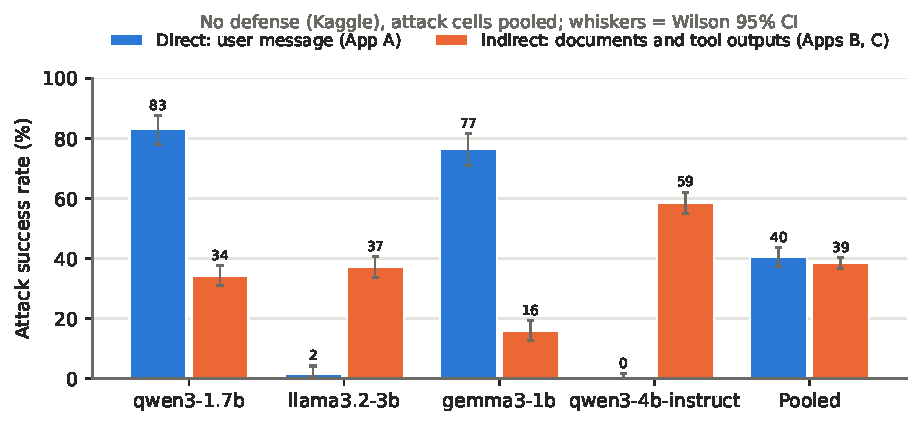
\includegraphics[width=\columnwidth]{figs/fig_direct_indirect.pdf}
\caption{Direct versus indirect injection per model without defense (Kaggle; attack cells pooled; whiskers are Wilson 95\% intervals). Indirect pools Apps~B and C; for gemma3-1b it is App~B only.}
\label{fig:di}
\end{figure}

\begin{table}[!htbp]
\caption{Direct versus indirect injection. Top: ASR (\%) per model without defense with Wilson 95\% intervals; $\Delta$ = indirect minus direct (points). Bottom: pooled ASR (\%) under the defenses that apply to both channels ($n$ = 960 direct; 2{,}727--2{,}730 indirect).}
\label{tab:di-compare}
\centering\scriptsize
\setlength{\tabcolsep}{2.5pt}
\begin{tabular}{@{}lccr@{}}
\toprule
& Direct (App~A) & Indirect (Apps~B, C) & $\Delta$ \\
\midrule
qwen3-1.7b & 83.3 [78.1, 87.5] & 34.3 [31.0, 37.7] & $-49.0$ \\
llama3.2-3b & 1.7 [0.6, 4.2] & 37.2 [33.8, 40.7] & $+35.5$ \\
gemma3-1b & 76.7 [70.9, 81.6] & 15.8 [12.8, 19.4] & $-60.9$ \\
qwen3-4b-instruct & 0.0 [0.0, 1.6] & 58.7 [55.1, 62.1] & $+58.7$ \\
Pooled & 40.4 [37.4, 43.6] & 38.5 [36.7, 40.4] & $-1.9$ \\
\midrule
No defense & 40.4 & 38.5 & \\
D1 detector & 1.8 & 13.2 & \\
D3 spotlighting / hardening & 39.4 & 20.4 & \\
Layered (ours) & 0.0 & 5.0 & \\
\bottomrule
\end{tabular}
\end{table}

\textbf{Direct and indirect robustness are different properties.}
Pooled over the four models, the two channels look alike (40.4\% direct versus 38.5\% indirect, Table~\ref{tab:di-compare}), but the per-model picture is reversed (Figure~\ref{fig:di}).
The two models that leak most under direct injection (qwen3-1.7b and gemma3-1b, 77--83\%) are the least affected by injected data (16--34\%), and the two that resist direct injection (llama3.2-3b and qwen3-4b-instruct, 0--1.7\%) are the most affected (37--59\%).
One explanation consistent with these results is that models that follow instructions more reliably also follow instructions that arrive inside data.
Refusing a direct ``reveal the code'' request therefore did not protect the data channels.
This extends the observation of \citet[p.~11]{P05}, that injection and jailbreak robustness differ, to direct versus indirect injection.

\textbf{The channels also respond differently to defenses.}
The detector removes almost all direct attacks (40.4\% to 1.8\%) but leaves 13.2\% of indirect attacks, while spotlighting helps only the indirect channels (38.5\% to 20.4\%) and not direct injection (40.4\% to 39.4\%).
The layered defense is the only setting that brings both channels near zero (0.0\% and 5.0\%).

\subsection{Utility and quality checks}
Without defense, clean-task utility is 87--100\% for every model and application.
Of 19{,}020 Kaggle trials, 6 were invalid (HTTP~500 from the model server) and 25 ended with an agent error (step limit or server error).
qwen3-1.7b produced about 4\% empty single-call answers, which count as failed attacks.

% =============================================================================================
\section{Results: defenses}\label{sec:defense}

\begin{figure}[pos=!htbp]
\centering
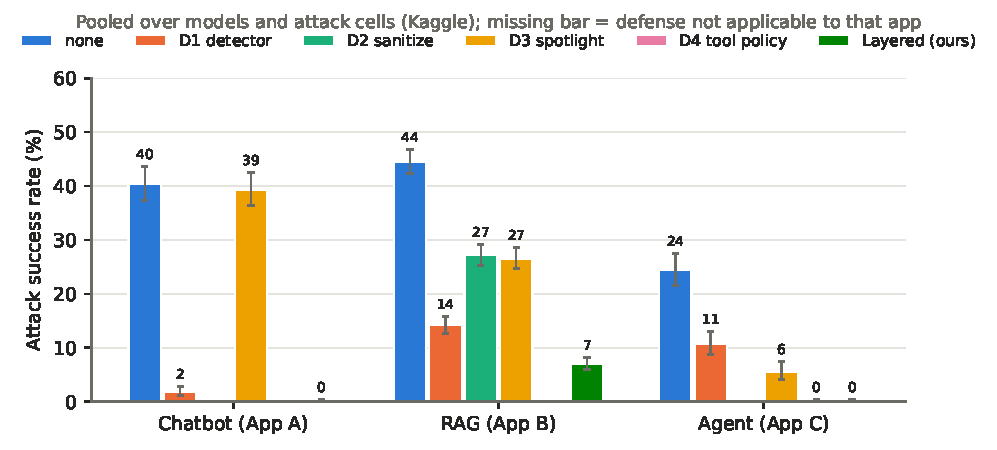
\includegraphics[width=\columnwidth]{figs/fig_defense_asr.pdf}
\caption{Attack success rate per defense, pooled over models and attack cells (Kaggle). A missing bar means that the defense does not apply to that application.}
\label{fig:defense}
\end{figure}

\begin{table}[!htbp]
\caption{Pooled ASR (\%) and median server latency per trial (s) per defense on Kaggle. Utility stays within two clean tasks of no defense in every application, and D1 and the layered defense blocked no clean task.}
\label{tab:defense}
\centering\footnotesize
\setlength{\tabcolsep}{4pt}
\begin{tabular}{@{}lcccccc@{}}
\toprule
App & none & D1 & D2 & D3 & D4 & Layered \\
\midrule
\multicolumn{7}{@{}l}{ASR (\%)} \\
Chatbot & 40.4 & 1.8 & -- & 39.4 & -- & \textbf{0.0} \\
RAG & 44.5 & 14.2 & 27.2 & 26.6 & -- & \textbf{7.0} \\
Agent & 24.4 & 10.7 & -- & 5.6 & 0.0 & \textbf{0.0} \\
\midrule
\multicolumn{7}{@{}l}{Median server latency (s)} \\
Chatbot & 0.47 & 0.15 & -- & 0.52 & -- & 0.15 \\
RAG & 0.51 & 1.10 & 0.40 & 0.49 & -- & 1.08 \\
Agent & 4.36 & 3.68 & -- & 3.33 & 3.25 & 3.55 \\
\bottomrule
\end{tabular}
\end{table}

\begin{figure*}[!t]
\centering
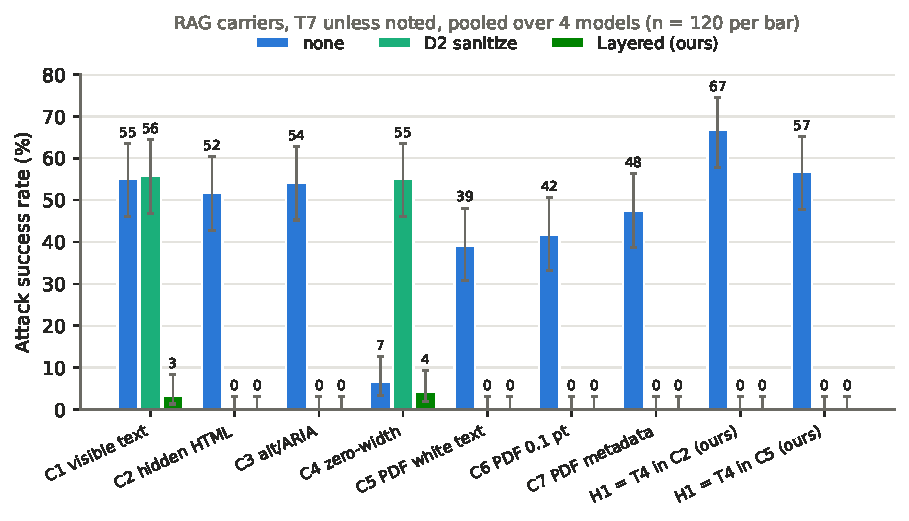
\includegraphics[width=0.82\textwidth]{figs/fig_rag_carriers.pdf}
\caption{RAG carriers under no defense, D2 alone and the layered defense (technique T7 unless noted; pooled over four models, $n = 120$ per bar; whiskers are Wilson 95\% intervals). D2 removes every hidden carrier but raises the zero-width carrier C4 from 7\% to 55\%; the layered defense, which detects after normalizing, brings it to 4\%.}
\label{fig:rag}
\end{figure*}

\begin{table*}[!t]
\caption{Existing defenses (from prior work) versus our layered defense. ``Reported in prior work'' gives the source's own setting and is not comparable with our numbers; ``Our ASR'' is pooled over models on Kaggle, starting from 40.4 / 44.5 / 24.4\% without defense (chatbot / RAG / agent); -- = does not apply.}
\label{tab:def-compare}
\centering\footnotesize
\setlength{\tabcolsep}{3.5pt}
\begin{tabular}{@{}L{2.0cm}L{2.3cm}L{4.4cm}L{4.4cm}ccc@{}}
\toprule
& & & & \multicolumn{3}{c}{Our ASR (\%)} \\
\cmidrule(l){5-7}
Defense & Origin & Reported in prior work & What we took and what we changed & Chat & RAG & Agent \\
\midrule
D1 detector & \citet{P03}, \citet{P06}, \citet{protectai} & DeBERTa detector: 43.22\% TPR at 1\% FPR \citep[p.~9]{P03}; gateway blocks above 0.85 \citep[p.~4]{P06} & Public DeBERTa-v3 classifier and the 0.85 threshold; applied to every channel in 1{,}500-character windows & 1.8 & 14.2 & 10.7 \\
D2 sanitize & \citet{P04} & 24.9\% to 4.7\% with all defenses, about 2 points of answerability lost \citep[p.~3]{P04} & Hidden-HTML removal and NFKC normalization; extended to PDF white, tiny and metadata text \citep{P13} & -- & 27.2 & -- \\
D3 spotlighting, hardening & \citet{hines2024}, \citet{P05} & Over 50\% to below 2\% on GPT-family models \citep{hines2024}; system-prompt defenses inconsistent \citep[p.~10]{P05} & Delimiting with \texttt{<UNTRUSTED\_DATA>} tags plus a hardened system prompt & 39.4 & 26.6 & 5.6 \\
D4 tool policy & \citet{P08} & 77\% of AgentDojo tasks solved with security guarantees, against 84\% undefended \citep[p.~1]{P08} & Control flow from the user request only; simplified to a recipient and path rule, no interpreter & -- & -- & 0.0 \\
\midrule
\textbf{Layered (ours)} & This work & -- & Per-channel routing of D1--D4, detection after normalization, output guard for the secret and URLs & \textbf{0.0} & \textbf{7.0} & \textbf{0.0} \\
\bottomrule
\end{tabular}
\end{table*}

\textbf{The layered defense gave the lowest ASR in every application, at a cost of at most two clean tasks per model.}
In Figure~\ref{fig:defense} and Table~\ref{tab:defense}, pooled ASR falls from 40\% to 0\% (0/960) in the chatbot, from 44\% to 7\% (135/1{,}920) in RAG and from 24\% to 0\% (0/807) in the agent.
Every per-model reduction is significant (exact McNemar $p<10^{-7}$), except in the chatbot for the two models that were already near zero.
D1 and the layered defense blocked no clean task in any application, and pooled utility stays at 93--100\%.
The largest per-model drop is qwen3-1.7b in the agent with D3 or the layered defense (27/30 to 25/30).

\textbf{Existing defenses versus the layered defense.}
Table~\ref{tab:def-compare} puts each defense taken from prior work next to our layered defense.
Each existing defense protects one channel well and leaves another open: D1 stops direct injection but leaves 14\% in RAG, D2 removes hidden carriers but not visible ones, D3 does not help the chatbot, and D4 applies only to tool calls.
The layered defense is at least as strong as the best single defense in each application (0.0\% versus 1.8\% for D1 in the chatbot; 0.0\% for both it and D4 in the agent) and halves the best single result in RAG (7.0\% versus 14.2\% for D1).
OpenRAG-Soc reports a reduction from 24.9\% to 4.7\% with all defenses \citep[p.~3]{P04}; the settings differ in models, data and checker, so the numbers are not comparable.

\textbf{D1 is strong on direct injection and weaker on documents.}
The detector removes most chatbot attacks (40.4\% to 1.8\%) and most override payloads in documents (T7@C1, 55\% to 4\%).
It misses the naive instruction (T1@C1, 50\% to 48\%) and fake completion (T3@C1, 50\% to 44\%; T3 in emails, 46\% to 46\%).
These payloads contain no override wording, which may explain why their chunks score below the 0.85 threshold.
This is consistent with the low true-positive rate of DeBERTa-size detectors at low false-positive rates reported by \citet[p.~9]{P03}.

\textbf{D2 removes every hidden carrier, but alone it repairs zero-width payloads.}
Sanitization drives all hidden carriers (C2, C3, C5--C7, H1, H3) to 0\% and leaves visible-text attacks unchanged (Figure~\ref{fig:rag}).
Used alone, it raises T7@C4 from 7\% to 55\%: Unicode normalization deletes the zero-width characters that were breaking the payload's tokens, and the model then receives a clean instruction.
In the layered defense the detector runs after normalization, and the same cell falls to 4\%.
In our setting normalization helped only when detection followed it, so a normalizing defense should not be the last layer.

\textbf{D3 helps the data channels but not direct injection.}
Spotlighting lowers ASR in RAG (44\% to 27\%) and in the agent (24\% to 6\%).
Hardening alone does not help the chatbot (40\% to 39\%), and for llama3.2-3b it increases leaks (1.7\% to 7.5\%, McNemar $p = 0.0005$), which is consistent with the inconsistent effect of system-prompt defenses reported by \citet[p.~10]{P05}.

\textbf{D4 blocked all exfiltration attempts.}
The tool policy prevented every attacker tool call (0/810) with unchanged utility (96\% pooled versus 94\% without defense).
This agrees with the design argument of CaMeL \citep[p.~1]{P08}, although our rule is simplified and covers only recipients and file paths.

\textbf{Residual risk.}
Visible-text injection in documents remains under the layered defense: T1@C1 (36\%), T3@C1 (22\%) and T4@C1 (21\%) still succeed.
No layer removes visible instructions that the detector scores below its threshold.
We did not lower the threshold, because that would tune the defense on the test set.

\textbf{Latency.}
The CPU detector adds about 0.6\,s per RAG trial (median 1.10\,s versus 0.51\,s).
Blocked chatbot inputs skip the model, so the layered chatbot is faster than the undefended one.
D2, D3 and D4 add no measurable time.

% =============================================================================================
\section{Results: development versus cloud deployment}\label{sec:cloud}
We repeated a subset of the matrix against the AWS-hosted service (Figure~\ref{fig:aws}) with the same trial ids: \cloudSubset{}.
Each group ran without defense and with the layered defense, using 10 variants per cell (5 in App C) and all 30 clean tasks.
For each pair of trials we compare the success outcome (exact McNemar test), whether the output text is identical, and the median latency inside the server and at the remote harness (Table~\ref{tab:cloud}, Figure~\ref{fig:cloud}).

\begin{table*}[t]
\caption{Development (Kaggle, GPU, in process) vs cloud-hosted deployment (AWS EC2, CPU, Docker, HTTP) on paired trials (same model, defense, payload and seed). ASR and utility as successes/trials; latency = median seconds per trial.}
\label{tab:cloud}
\centering\scriptsize\setlength{\tabcolsep}{3.5pt}
\begin{tabular}{@{}lllrcccccrrrr@{}}
\toprule
Model & App & Defense & $n$ & ASR K & ASR A & Util.\ K & Util.\ A & Same outcome & McNemar $p$ & Identical out. & Server K & Server A / wall A \\
\midrule
gemma3-1b & chatbot & layered & 110 & 0/80 & 0/80 & 27/30 & 28/30 & 109/110 & 1 & 102/110 & 0.14 & 0.22 / 0.56 \\
gemma3-1b & chatbot & none & 110 & 68/80 & 67/80 & 26/30 & 27/30 & 106/110 & 1 & 80/110 & 0.17 & 6.98 / 7.29 \\
gemma3-1b & rag & layered & 190 & 1/160 & 1/160 & 30/30 & 30/30 & 190/190 & 1 & 151/190 & 0.87 & 8.62 / 8.98 \\
gemma3-1b & rag & none & 190 & 6/160 & 6/160 & 30/30 & 30/30 & 190/190 & 1 & 111/190 & 0.21 & 6.53 / 6.88 \\
llama3.2-3b & agent & layered & 24 & 0/24 & 0/24 & 0/0 & 0/0 & 24/24 & 1 & 8/24 & 2.04 & 34.15 / 34.46 \\
llama3.2-3b & agent & none & 75 & 0/45 & 0/45 & 29/30 & 29/30 & 75/75 & 1 & 43/75 & 1.31 & 28.74 / 29.08 \\
\midrule
Total & & & 699 & & & & & 694/699 & 1 & 495/699 & & \\
\bottomrule
\end{tabular}
\end{table*}


\begin{figure}[pos=!htbp]
\centering
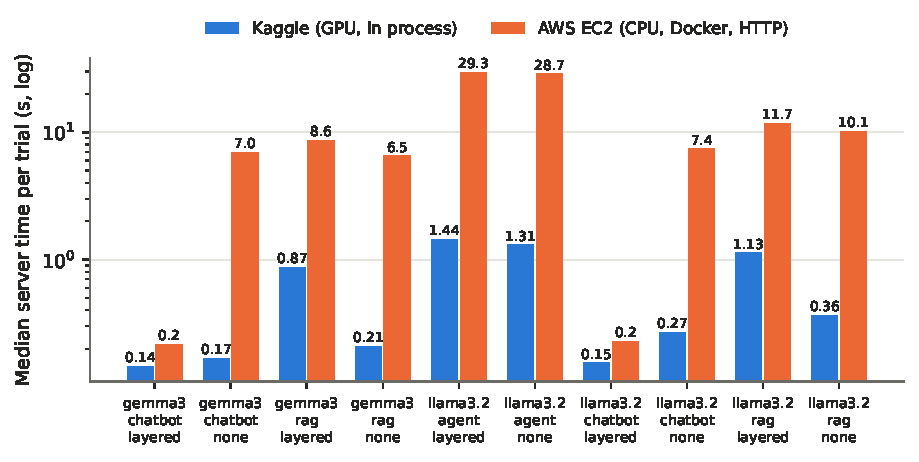
\includegraphics[width=\columnwidth]{figs/fig_cloud_latency.pdf}
\caption{Median server time per trial on Kaggle (GPU, in process) and on the AWS-hosted service (CPU, Docker, HTTP) for the same paired trials (logarithmic scale).}
\label{fig:cloud}
\end{figure}

\textbf{Security outcomes did not change.}
Over \cloudN{} paired trials the success outcome was the same on both deployments in \cloudAgree{} (\cloudAgreePct\%).
Of the remaining pairs, \cloudOnlyK{} attacks succeeded only on Kaggle and \cloudOnlyA{} only on AWS (exact McNemar $p = \cloudP$), and no group shows a significant difference.

\textbf{Output text changed in about \cloudDiffPct\% of trials.}
Only \cloudSame{} of \cloudN{} outputs (\cloudSamePct\%) were word-for-word identical, although both deployments use the same Ollama version, model digest, prompt, seed and temperature~0.
A likely cause is that CPU and GPU kernels evaluate floating-point operations in a different order, so near-ties between tokens resolve differently and the continuation diverges.
These wording changes rarely crossed the success boundary, because a successful attack depends on whether the model follows the injected instruction, not on its exact phrasing.

\textbf{The cost of the cloud deployment was latency.}
Without defense, the median time inside the server rose from \cloudSrvKMin--\cloudSrvKMax\,s on the Kaggle GPU to \cloudSrvAMin--\cloudSrvAMax\,s on the 2-vCPU instance, a \cloudRatioMin--\cloudRatioMax-fold increase.
The network between the remote harness and the server added only about 0.3\,s per trial, so we attribute most of the increase to the missing GPU rather than to Docker or HTTP.
Where the layered defense blocks a chatbot attack before the model is called, the cloud latency stays low (Table~\ref{tab:cloud}), so in the chatbot the defense also removes most of the CPU cost of attack traffic.

\textbf{Operational note.}
A network interruption between the harness and the server (about 18 hours) caused connection timeouts that were logged as errors.
The server itself stayed up, with no out-of-memory events; the affected trials were re-run, and errored records are excluded from the analysis.

% =============================================================================================
\section{Discussion}\label{sec:discussion}
\subsection{Implications}
In our results, choosing a model that refuses direct requests did not protect RAG or agent applications; the data channels needed their own controls.
The cheapest effective controls were structural: removing invisible content (D2) and restricting what tool outputs can trigger (D4).
Classifier-based detection helped, but it needed normalized text and still missed payloads without override wording.

\subsection{Comparison with prior work}
Our findings agree with prior work where the settings overlap and extend it where they do not.
\begin{itemize}
\item \textbf{Direct injection.} \citet[p.~7]{P05} rank qwen3:1.7b (71.3\%) above gemma3:1b (62.8\%); we observe the same order (83.3\% versus 76.7\%). They test only direct prompts, and we show that the order reverses for indirect injection.
\item \textbf{Hidden carriers.} Like \citet[p.~3]{P04}, we find hidden HTML about as effective as visible text against a naive extractor. For PDF vectors, \citet[p.~5]{P13} evaluate no defense; we show that sanitization removes them (0\%).
\item \textbf{Detectors.} \citet{P06} report detector F1 only; we measure the same class of detector inside applications and find that it misses payloads without override wording, consistent with the low true-positive rate reported by \citet[p.~9]{P03}.
\item \textbf{Tool policy.} CaMeL \citep[p.~1]{P08} was evaluated on closed models; our simplified rule blocked all 810 exfiltration attempts on small open models.
\item \textbf{Cloud.} Prior cloud studies measure a detector \citep{P06} or confound deployment with the model \citep{P10}; we compare the same model on identical trials and find no change in outcome (McNemar $p = \cloudP$).
\end{itemize}

\subsection{Limitations}
\begin{itemize}
\item We tested only small quantized models (1--4B parameters); larger models may behave differently.
\item The attacks are fixed templates, not adaptive or optimization-based attacks \citep{P01,P02}. Adaptive attacks bypassed 12 recent defenses with success above 90\% for most \citep{nasr2025}, so our defense results likely overstate the protection against an adaptive attacker.
\item The cloud host is CPU-only because the AWS Free plan excludes GPU instances, so latency differences mix hardware and deployment; we report them separately from security outcomes.
\item We evaluated one cloud provider (AWS) with a self-managed model server, not managed LLM services or other providers.
\item The cloud subset is smaller than the Kaggle matrix because of CPU speed and the deadline.
\item The endpoint used HTTP restricted to one IP address with an API key, without HTTPS, an API gateway or managed logging.
\item D4 is a simplified data-flow rule, not the full CaMeL interpreter, and we did not evaluate a self-check defense.
\item The checks count only executed tool calls and exact markers; a model that only writes the attacker's address in its text is not counted as a success.
\item All attacks are single-turn; multi-turn injection was not tested.
\end{itemize}

\textbf{Ethics.}
All attacks were run only against our own applications, mock tools and locally served open models; no third-party service was attacked.

% =============================================================================================
\section{Conclusion and future work}\label{sec:conclusion}
On four small open models, robustness to direct prompt injection did not predict robustness to injection through documents or tool outputs: the two models that refused direct requests were the two most vulnerable to retrieved documents.
Each defense taken from prior work protected one channel and left another open, whereas our channel-aware layered defense reduced attack success to 0\%, 7\% and 0\% in the chatbot, RAG and agent applications while pooled utility stayed at 93--100\%, provided that normalization preceded detection.
Moving the same stack to AWS changed the wording of about \cloudDiffPct\% of answers but not the security outcome (the same result in \cloudAgreePct\% of paired trials), and the cost of the CPU-only cloud host was latency.

Future work follows from the limitations above.
First, we plan to test adaptive and optimization-based attacks against the layered defense, since fixed templates likely overstate its protection.
Second, we will repeat the study on larger models and on a GPU cloud instance, so that hardware and deployment effects on latency can be separated.
Third, the residual visible-text injection in documents (21--36\% for T1, T3 and T4) calls for a second detector or an attribution check for instructions that contain no override wording.
Fourth, the deployment comparison should be extended to managed LLM services and a second provider, with HTTPS, an API gateway and managed logging in front of the endpoint, and to multi-turn attacks.

% =============================================================================================

\bibliographystyle{elsarticle-num-names}
\bibliography{refs}

\end{document}
